\subsection{Introduction}
Optical communication systems are integral to modern telecommunication networks, and equalization techniques play a vital role in mitigating signal impairments caused by dispersion and nonlinearity effects. Traditional equalization methods, such as linear filtering or digital backpropagation may not always deliver optimal performance for highly nonlinear systems\cite{essiambre2012capacity, cartledge2017digital, bayvel2016maximizing}. Consequently, alternative approaches, including machine learning techniques, have been explored to address the equalization challenge in optical communication systems\cite{zibar2015machine, freire2021performance}.

Gradient boosting (GB), a powerful ensemble learning method, has emerged as a promising equalization technique for optical communication systems due to its adaptability and ability to model complex input-output relationships\cite{Chen:2016:XST:2939672.2939785,natekin2013gradient,friedman2002stochastic,bentejac2021comparative}. This technique combines multiple weak learners, typically decision trees, to create a strong learner by iteratively training decision trees to correct the errors of their predecessors. By minimizing a loss function through a gradient descent-like optimization, gradient boosting gradually improves the accuracy of its predictions.

One of the advantage of gradient boosting is its robustness to overfitting. By employing techniques such as shrinkage, regularization, and early stopping, gradient boosting can effectively prevent overfitting, even when dealing with high-dimensional data. Furthermore, gradient boosting is inherently parallelizable, allowing for efficient implementations on modern hardware architectures, including multi-core CPUs, GPUs, and even FPGAs\cite{alcolea2021fpga}. The compatibility with FPGAs can offer low-latency and power-efficient solutions, which are particularly important for real-time applications in optical communication systems.

Gradient boosting also outperforms other tree-based ensemble methods like random forests in terms of predictive accuracy\cite{natekin2013gradient}. While random forests build trees independently and rely on bagging to reduce overfitting, gradient boosting builds trees sequentially and focuses on minimizing the errors made by previous trees. This sequential approach enables gradient boosting to adapt more effectively to the data, ultimately leading to better performance in many applications.

In terms of complexity, gradient boosting can be more computationally efficient compared to other machine learning techniques such as deep learning, which often requires extensive training time, large amounts of data, and significant hardware resources. The relative simplicity of the decision trees used in gradient boosting and the flexibility in controlling the ensemble size allow for better control over the trade-off between complexity and performance, making it a suitable choice for various scenarios in optical communication systems.

In this paper, we explore the application of gradient boosting as a novel equalization technique in optical communication systems, focusing on its potential to surpass the performance of traditional equalization methods. By harnessing the power of the gradient boosting algorithm, we aim to achieve increased predictive performance while simultaneously reducing the computational complexity of the equalization process. This innovative approach positions gradient boosting as a promising candidate for equalization tasks in optical communication systems, with the potential to outperform conventional techniques and pave the way for future advancements in the field.


\subsection{Methodology}


\begin{figure*}[ht]
   \centering
    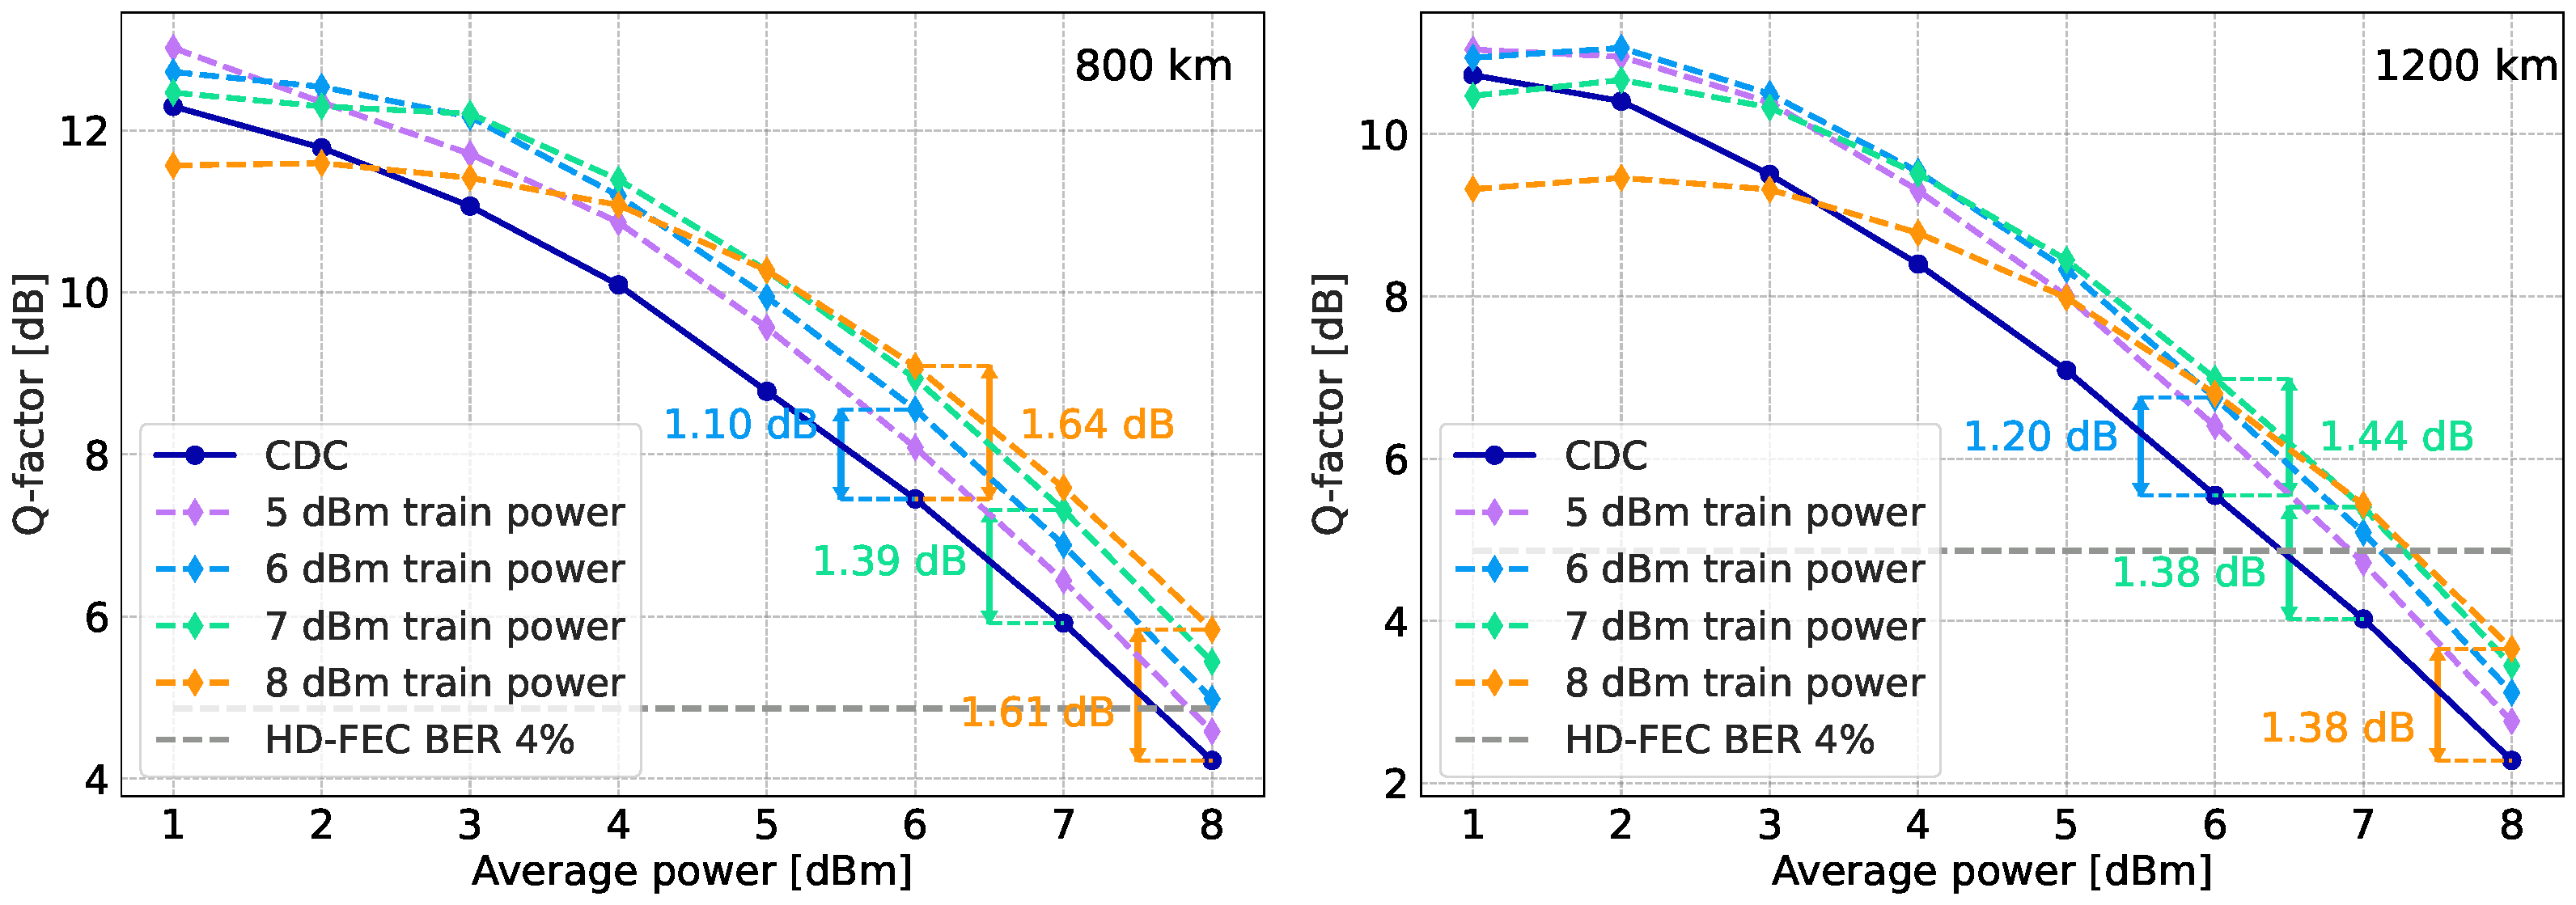
\includegraphics[width=1\linewidth]{images/boost/q_different_models_couple.pdf}
    \caption{Q-Factor performance after nonlinear equalization using GB trained at varying average signal power levels. Solid lines represent the system with CDC, and horizontal dashed lines indicate the HD-FEC threshold for a BER of 4\%. Total propagation distance of 800 km \textbf{(left)}, and 1200 km \textbf{(right)}.}
    \label{fig:fig1}
\end{figure*}

\begin{figure}[ht]
   \centering
        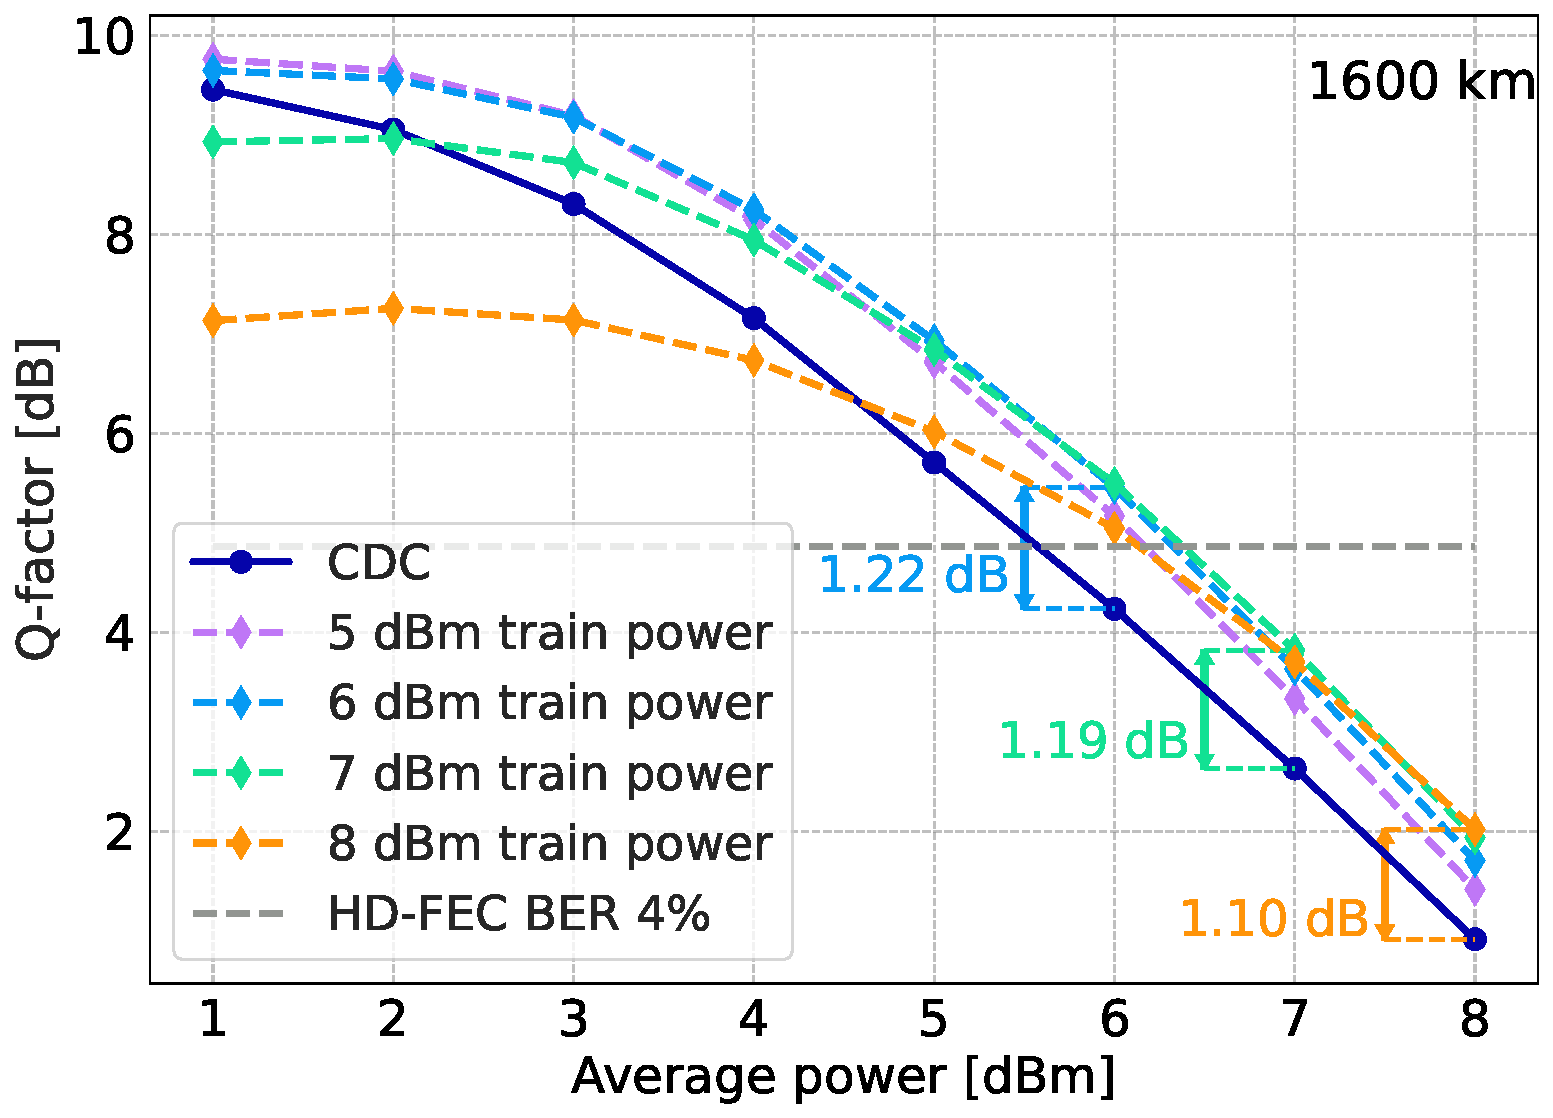
\includegraphics[width=0.5\linewidth]{images/boost/q_different_models_single.pdf}
    \caption{Analogous to Fig.~\ref{fig:fig1}, Q-Factor performance for a total propagation distance of 1600 km, after nonlinear equalization using GB trained at different average signal power levels.}
    \label{fig:fig2}
\end{figure}

In this study, we introduce a novel approach to nonlinear equalization in optical communication systems by employing a GB algorithm based on decision trees.
We used an optical channel model of standard single-mode fiber (SSFM) with erbium-doped fiber amplifiers (EDFAs) and varying transmission distances, including 10, 15, and 20 spans of 80 km each. The signal format is a 16-quadrature amplitude modulation (16-QAM) WDM with dual polarization and a symbol rate of $34.4\;\textrm{GBd}$. The pulse shaping employed a digital root-raised cosine (RRC) filter with a roll-off factor of $0.1$. The transmission distance varied between $10$, $15$, and $20$ spans of $80\;\textrm{km}$ each, with EDFA amplification. The EDFA noise figure was set at $4.5\;\textrm{dB}$. The average signal power range was from $1$ to $8\;\textrm{dBm}$, but for training, we used power from $4\;\textrm{dBm}$ to $8 \textrm{dBm}$. The signal propagation through the fiber was represented by a generalized Manakov equation using the GPU-accelerated split-step Fourier method\cite{esf0_2023_7880552}. The fiber parameters included a wavelength of $\lambda = 1550\;\textrm{nm}$, a dispersion coefficient of $D = 16.8\;\textrm{ps}/(\textrm{nm} \cdot \textrm{km})$, and a nonlinear coefficient of $\gamma = 1.2\;\textrm{W}^{-1} \cdot \textrm{km}^{-1}$.

We generated around $10$ million datapoints for each specific average power and propagation distance. The dataset was then divided into training and test sets, with the test set comprising $1\%$ of the full dataset (about $100,000$ points).

In the dataset used for training, the input consists of values of the received points for the x-polarization, for which we aim to predict the nonlinear shift. To account for the neighboring points' influence, we include five values of received points to the right and left of the central point (neighbors in the sequence of points). Since we utilize two polarizations, we also incorporate the central point for y-polarization (in the same position in the sequence as for x-polarization) and its five neighboring points on both the left and right. As a result, a total of 22 complex points serve as input for the GB algorithm. The output represents the nonlinear shift (a complex number that must be added to accurately shift the point to its original position in the constellation) for the received point in the x-polarization.

The gradient boosting algorithm was implemented using the XGBoost library\cite{Chen:2016:XST:2939672.2939785} with GPU acceleration. The training process involved a large number of estimators, specifically $200,000$, which were chosen to test the idea of using decision trees but can be significantly reduced for a particular system. The maximum tree depth did not exceed $20$, the learning rate was set to $0.1$, and the $L_2$ and $L_1$ regularization parameters were both set to $1.0$.

\subsection{Complexity}
The complexity of prediction for gradient boosting can be expressed using the following formula:
$$
C(GB) = N_{trees} \cdot M \cdot N_{features}
$$
where $C(GB)$ represents the complexity of prediction for gradient boosting, $N_{trees}$ is the number of trees in the ensemble, $M$ is the maximum depth of each tree, $N_{features}$ is the number of features in the dataset.

This formula assumes that the complexity of each decision in the tree is constant and that the trees have a balanced structure. In practice, the trees might not be perfectly balanced, and the actual complexity could be somewhat lower. However, this formula provides a useful estimate for understanding the relationship between the main parameters of gradient boosting and its prediction complexity.

At first glance, it may appear that the overall complexity for our chosen set of parameters is excessively high. In this study, our primary goal is not to achieve cutting-edge complexity but rather to demonstrate the proof-of-concept. However, it is important to emphasize that each parameter contributing to complexity can be optimized to significantly reduce the overall complexity. Comprehensive information about feature importance allows us to manage input parameters (which can be further reduced) and to control the impact of each decision tree, thereby enabling the removal of unnecessary trees to enhance performance. Moreover, we can manually regulate the maximum depth of each tree, which, after optimization, can ultimately yield the desired performance.

\subsection{Results}
To demonstrate the potential of GB, we assessed the performance of various GB models across a range of propagation distances and diverse input signal average powers. The results were analyzed in terms of Q-factor improvement and the level of HD-FEC (Hard Decision Forward Error Correction), which represents a common error correction scheme used in optical communication systems. The target Bit Error Rate (BER) was set at $4\%$.

For all propagation distances, the GB models showed at least a $1\;\textrm{dB}$ improvement in Q-factor compared to the system with Chromatic Dispersion Compensation (CDC). Specifically, for a $1600\;\textrm{km}$ transmission distance (Fig.~\ref{fig:fig2}), the model trained on $8\;\textrm{dBm}$ signals exhibited a $1.10\;\textrm{dB}$ improvement in Q-factor for the same test power. The model trained on $7\;\textrm{dBm}$ signals displayed a $1.19\;\textrm{dB}$ improvement for the same test power, while the model trained on $6\;\textrm{dBm}$ signals showed a $1.22\;\textrm{dB}$ improvement. The $1.22\;\textrm{dB}$ Q-factor improvement for the $6\;\textrm{dBm}$ model allowed us to decrease the BER (increase the Q-factor) below (above) the HD-FEC level.

Interestingly, models trained on higher average power (and thus experiencing higher nonlinear distortions) exhibited good performance when applied to lower test power levels. However, their performance degraded for higher test power levels. This observation suggests that the GB algorithm can successfully mitigate nonlinear effects. This is particularly evident in Fig.~\ref{fig:fig1} (left) for a propagation distance of $800\;\textrm{km}$. The model trained on $8\;\textrm{dBm}$ outperformed other models for power levels from $5\;\textrm{dBm}$ to $8\;\textrm{dBm}$, showing approximately $1.6\;\textrm{dB}$ improvement (specifically, $1.64\;\textrm{dB}$ for $6\;\textrm{dBm}$ test power and $1.61\;\textrm{dB}$ for $8\;\textrm{dBm}$ test power). For $8\;\textrm{dBm}$, the improved Q-factor surpassed the HD-FEC level. However, for lower signal powers, the model trained on $8\;\textrm{dBm}$ performed poorly, since these regimes are less influenced by nonlinear effects.

A similar pattern can be observed in Fig.~\ref{fig:fig1} (right) for a propagation distance of $1200\;\textrm{km}$. In this case, the model trained on $7\;\textrm{dBm}$ showed significant improvement for a wide range of test signal powers (from $3\;\textrm{dBm}$ to $8\;\textrm{dBm}$). This finding indicates that the GB training power can be optimized for specific power ranges in which the system operates. The wide range of applicability allows for the development of a universal equalizer based on GB, which does not require retraining for different power levels (subject to the constraints of the working regime for GB).


\subsection{Conclusion}
In conclusion, this study has demonstrated the potential of gradient boosting as a novel equalization technique in optical communication systems, offering better predictive performance with the possibility of reduced complexity compared to traditional methods. This innovative approach may pave the way for advancements in the field and enhance the efficiency of modern telecommunication networks.

Future research should focus on optimizing the complexity-performance trade-off, investigating real-world robustness, and exploring hardware acceleration opportunities. Developing a universal equalizer based on gradient boosting could further expand the applicability of this technique in optical communication systems.